% !TEX TS-program = lualatex
\documentclass{beamer}
%\documentclass[slideopt,A4]{beamer}
\input{../common/misomva}
\usepackage{fontawesome5}
\usetikzlibrary{positioning, shapes.geometric, shapes.symbols, shadows, calc, shapes.callouts, fit, backgrounds}

\definecolor{bgDark}{HTML}{222b30}
\definecolor{bgLight}{HTML}{f0eee5}
\definecolor{boxOrange}{HTML}{ff9d6e}
\definecolor{boxBlue}{HTML}{9cbce2}
\definecolor{boxLightBlue}{HTML}{e1eaf5}
\definecolor{boxWhite}{HTML}{f0f5fa}
\definecolor{b2Box2}{HTML}{dbe4f0} 
\definecolor{b2Box3}{HTML}{99b6d9} 
\definecolor{b2Box4}{HTML}{eef2f7}
\definecolor{b3Box2}{HTML}{e1eaf5}
\definecolor{b3Box3}{HTML}{e1eaf5}
\definecolor{b3Box4}{HTML}{99b6d9}
\definecolor{calloutYellow}{HTML}{fffeb3}
\begin{document}
\newcommand{\misoclasstinytitleslide}{}
\newcommand{\misoclassdate}{}
\MakeTitleSlide

%\section{Where are the graphs coming from?}
\begin{frame}
\frametitle{\textbf{Two (main) sources of graphs in ML}}

%\begin{columns}
%\begin{column}{.5\textwidth}
\textbf{Natural graphs as models for networks}
\begin{itemize}\addtolength{\itemsep}{.25\baselineskip}
\item<2-> {given as an input} 
\item<3-> discover interesting properties of the structure
%\item represent useful information (viral marketing)
%\item is the object of study (anomaly detection)
\end{itemize}
%\end{column}
%\begin{column}{.5\textwidth}

%\pause
\vspace{\baselineskip}
\textbf{Constructed graphs as nonparametric basis}
\begin{itemize}\addtolength{\itemsep}{0.25\baselineskip}
\item<4-> we create (learn) the similarity structure from flat data
\item<5-> it's a tool (e.g., nonparametric regularizer) to encode structural properties (e.g., independence, $\dots$)
\end{itemize}
%\end{column}
%\end{columns}
\end{frame}

\begin{frame}
\frametitle{Natural graphs from \emphcol{social networks}}
\begin{columns}
\begin{column}{.5\textwidth}
\begin{itemize}[<+-| alert@+>]\addtolength{\itemsep}{1\baselineskip}
\item people and their interactions
\item structure is rather a \textit{phenomena}
\item typical ML tasks 
\begin{itemize}\addtolength{\itemsep}{0.5\baselineskip}
\item advertising 
%\item product placement 
\item link prediction (PYMK)
\item find influential sources 
\end{itemize}
\end{itemize}
\end{column}
\begin{column}{.5\textwidth}
\begin{center}
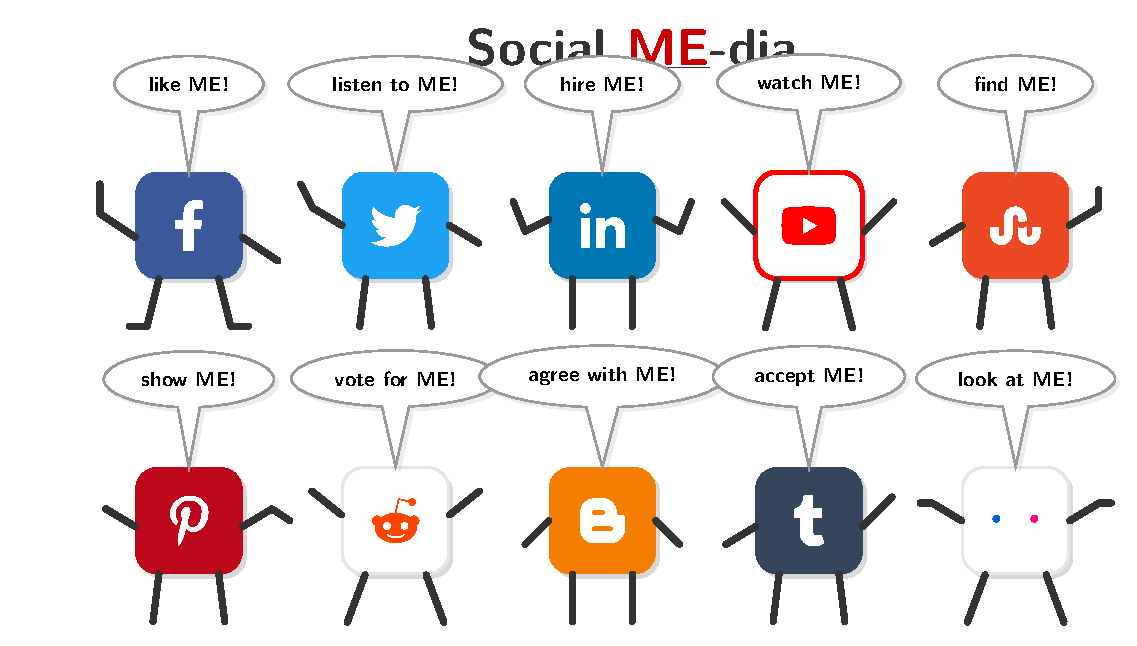
\includegraphics[width=\textwidth]{../img/mlapa-tikz-preview.pdf}
\end{center}
\vspace{0.2em}
{\tiny Source: Murphy (2012)}
\end{column}
\end{columns}
\end{frame}


\begin{frame}
\frametitle{Natural graphs from \emphcol{utility and technology networks}}
\begin{columns}
\begin{column}{.5\textwidth}
\begin{itemize}[<+-| alert@+>]\addtolength{\itemsep}{1\baselineskip}
%\item link services 
\item power grids, roads, Internet, sensor networks
\item structure is either \textit{hand designed} or not
\item typical ML tasks 
\begin{itemize}\addtolength{\itemsep}{0.5\baselineskip}
\item best routing under unknown or variable costs 
\item identify the node of interest  
\end{itemize}
\end{itemize}
\end{column}
\begin{column}{.5\textwidth}
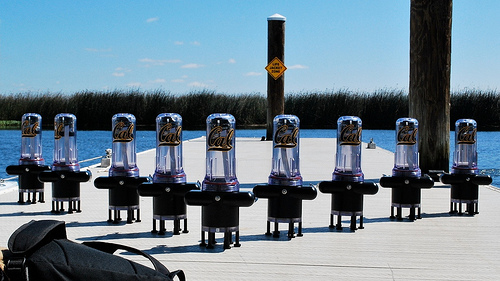
\includegraphics[width=\textwidth]{../img/berkelywatersensornetworks.jpg}\\
{\tiny Source: Guestrin et al. (2005)}
{\small Berkeley's Floating Sensor Network} 
\end{column}
\end{columns}
\end{frame}


%\begin{frame}
%\frametitle{Graphs from \emphcol{information networks}}
%\begin{columns}
%\begin{column}{.5\textwidth}
%\begin{itemize}[<+-| alert@+>]\addtolength{\itemsep}{1\baselineskip}
%\item web  
%\item blogs
%\item wikipedia
%\item typical ML tasks 
%\begin{itemize}\addtolength{\itemsep}{0.5\baselineskip}
%\item find influential sources 
%\item search (pagerank)  
%\end{itemize}
%\end{itemize}
%\end{column}
%\begin{column}{.5\textwidth}
%\begin{center}
%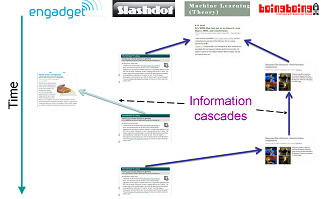
\includegraphics[width=\textwidth]{../img/cascade}\\
%{\tiny Blog cascades (ETH) - \emph{submodularity}} 
%\end{center}
%\end{column}
%\end{columns}
%\end{frame}



\begin{frame}
\frametitle{Natural graphs from \emphcol{biological networks}}
\begin{columns}
\begin{column}{.5\textwidth}
\begin{itemize}[<+-| alert@+>]\addtolength{\itemsep}{1\baselineskip}
\item protein-protein interactions  
\item gene regulatory networks
\item typical ML tasks 
\begin{itemize}\addtolength{\itemsep}{0.5\baselineskip}
\item discover unexplored interactions 
\item learn or reconstruct the structure
\end{itemize}
\end{itemize}
\end{column}
\begin{column}{.5\textwidth}
\begin{center}
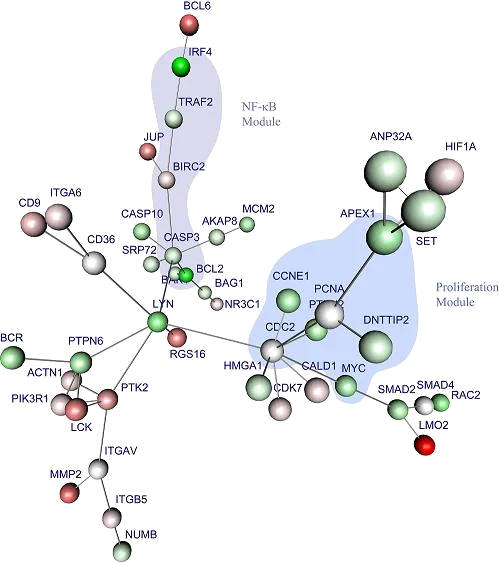
\includegraphics[width=\textwidth]{../img/bionetwork}\\
{\tiny Source: Basso et al. (2005)}
{\tiny Diffuse large B-cell lymphomas -  Dittrich et al. (2008)} 
\end{center}
\end{column}
\end{columns}
\end{frame}


\begin{frame}
\frametitle{Constructed graphs from \emphcol{similarity networks}}
\begin{center}%
\only<1|handout:1>{%
\textbf{graph is not naturally given}\\[1em]%
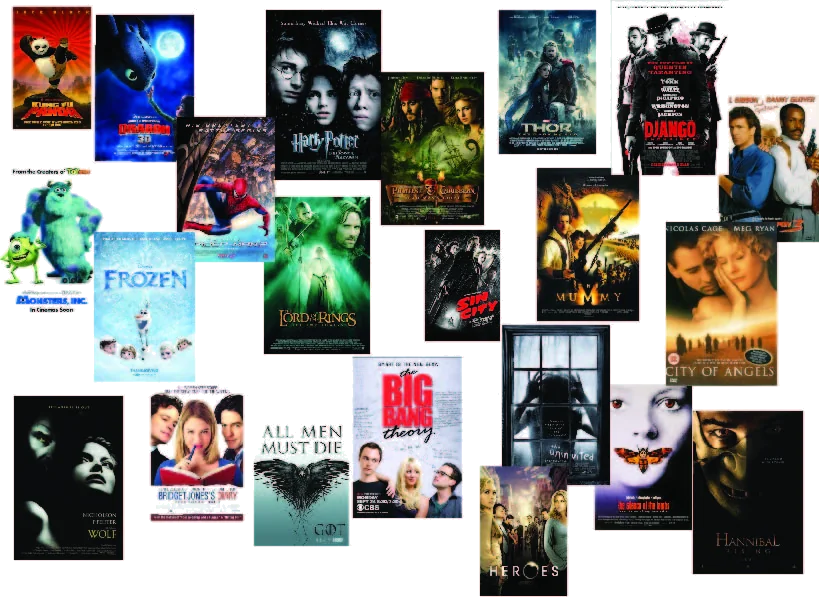
\includegraphics[width=0.8\columnwidth]{../img/movies1}}%
\only<2|handout:2>{%
\textbf{but we can construct it}\\[1em]%
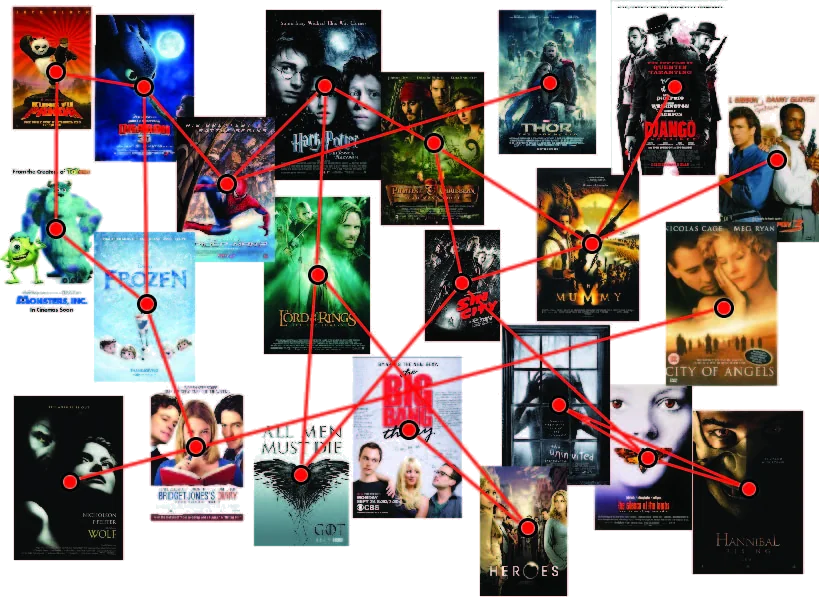
\includegraphics[width=0.8\columnwidth]{../img/movies2}}%
\only<3|handout:3>{%
\textbf{and use it as an abstraction}\\[1em]%
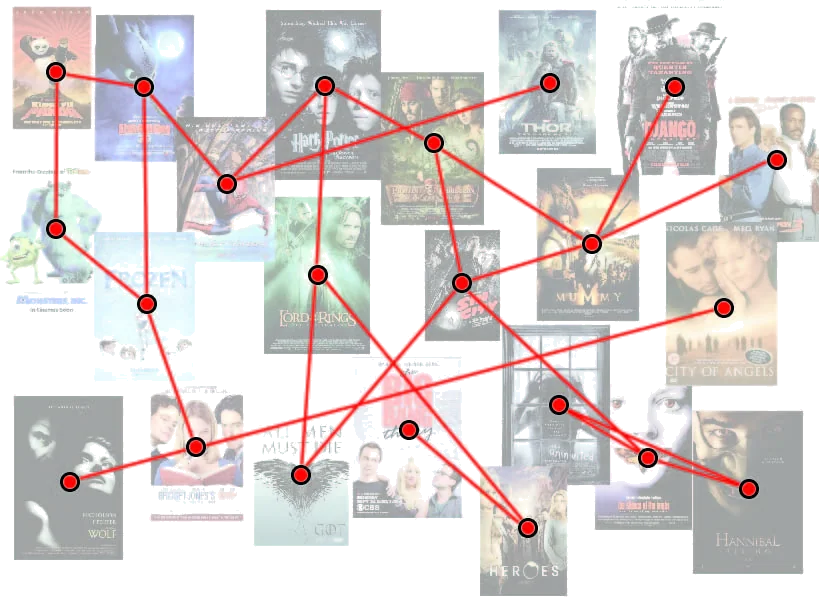
\includegraphics[width=0.8\columnwidth]{../img/movies3}\\
{\tiny Source: Movie posters collage}}%
\end{center}
\end{frame}

\begin{frame}
\frametitle{Constructed graphs from \emphcol{similarity networks}}
\begin{columns}
\begin{column}{.5\textwidth}
\begin{itemize}\addtolength{\itemsep}{1\baselineskip}
\item vision  
\item audio
\item text  
\onslide<2|handout:1>{
\item typical ML tasks 
\begin{itemize}\addtolength{\itemsep}{0.5\baselineskip}
\item semi-supervised learning  
\item spectral clustering  
\item manifold learning
\end{itemize}
}
\end{itemize}
\end{column}
\begin{column}{.5\textwidth}
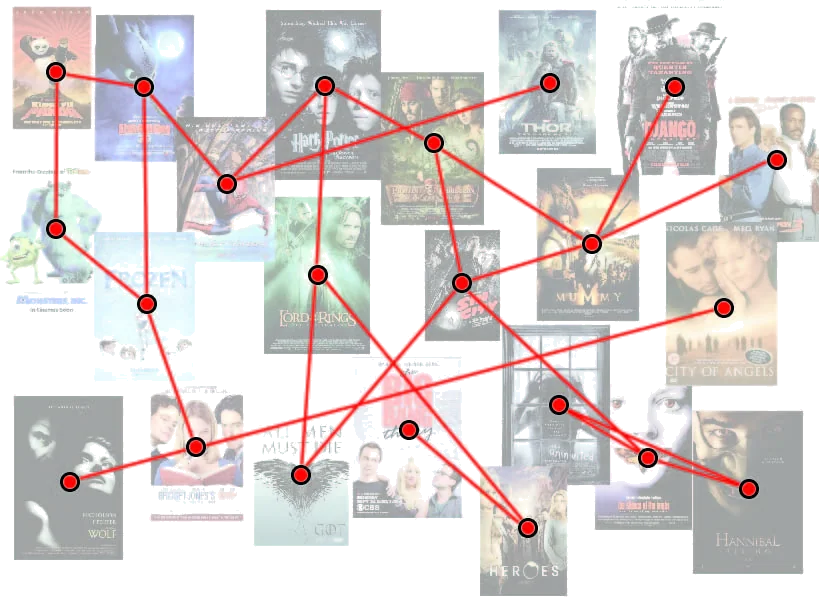
\includegraphics[width=\textwidth]{../img/movies3}\\
{\small Movie similarity} 
\end{column}
\end{columns}
\end{frame}





%\section{Random Graph Models}

%\begin{frame}
%\frametitle{\textbf{In between: random graph models}}
%\begin{columns}
%\begin{column}{.33\textwidth}
%\textbf{Erd\H os-R\' enyi}
%%\begin{itemize}\addtolength{\itemsep}{1\baselineskip}
%%\item 
%{\small independent edges} 
%\bigskip
%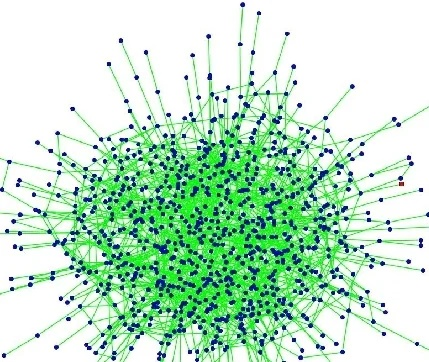
\includegraphics[width=0.9\textwidth]{../img/er}\\
%%\end{itemize}
%\end{column}
%%\pause
%\begin{column}{.33\textwidth}
%\textbf{Barab\'asi-Albert}
%\bigskip
%%\begin{itemize}\addtolength{\itemsep}{0.7\baselineskip}
%%\item 
%{\small preferential attachment}  
%%\end{itemize}
%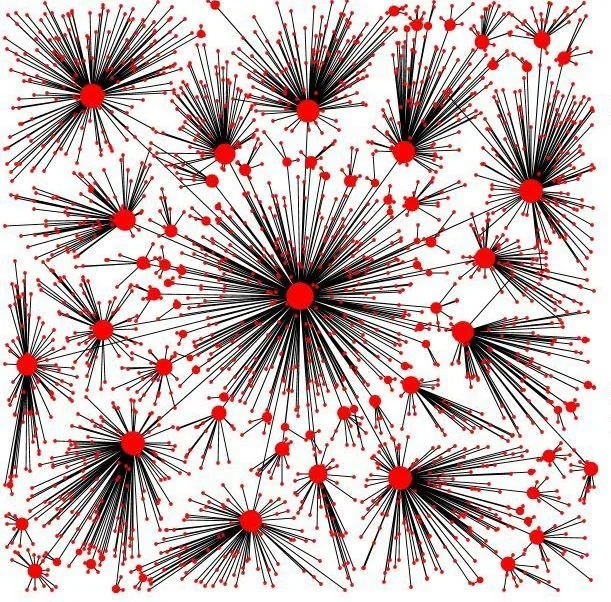
\includegraphics[width=0.8\textwidth]{../img/bamodel}\\
%\end{column}
%%\pause
%\begin{column}{.35\textwidth}
%\textbf{Stochastic Blocks}
%%\begin{itemize}\addtolength{\itemsep}{0.7\baselineskip}
%%\item 
%{\small modeling communities}  
%\bigskip
%%\end{itemize}
%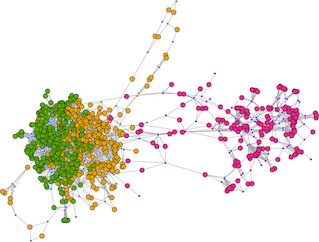
\includegraphics[width=\textwidth]{../img/sbm}\\
%\end{column}
%\end{columns}
%\bigskip
%%\pause
%Watts-Strogatz, Chung-Lu, Fiedler, \dots.

%\end{frame}

%\section{In this course}

\begin{frame}

\frametitle{\textbf{What will you learn in the Graphs in ML course?}}

\textbf{Concepts, tools, and methods} to work with graphs in ML.  \\[2em]

\pause Specific applications of graphs in ML. \\[2em]

\pause Theoretical toolbox to analyze graph-based algorithms.\\[2em]

\pause How to tackle: \emph{large graphs, online setting, graph construction} \dots  \\[2em]

\pause One example: \yellbox{Online Semi-Supervised Face Recognition} 

\end{frame}


%\section{Online SSL Face Recognition}

\begin{frame}
\frametitle{\textbf{Online Semi-Supervised Face Recognition}}
\begin{center}
\only<1,3|handout:1>{
\vspace{-1.5em}
\onslide<3>{\textbf{graph is not given\\[1em]}}%
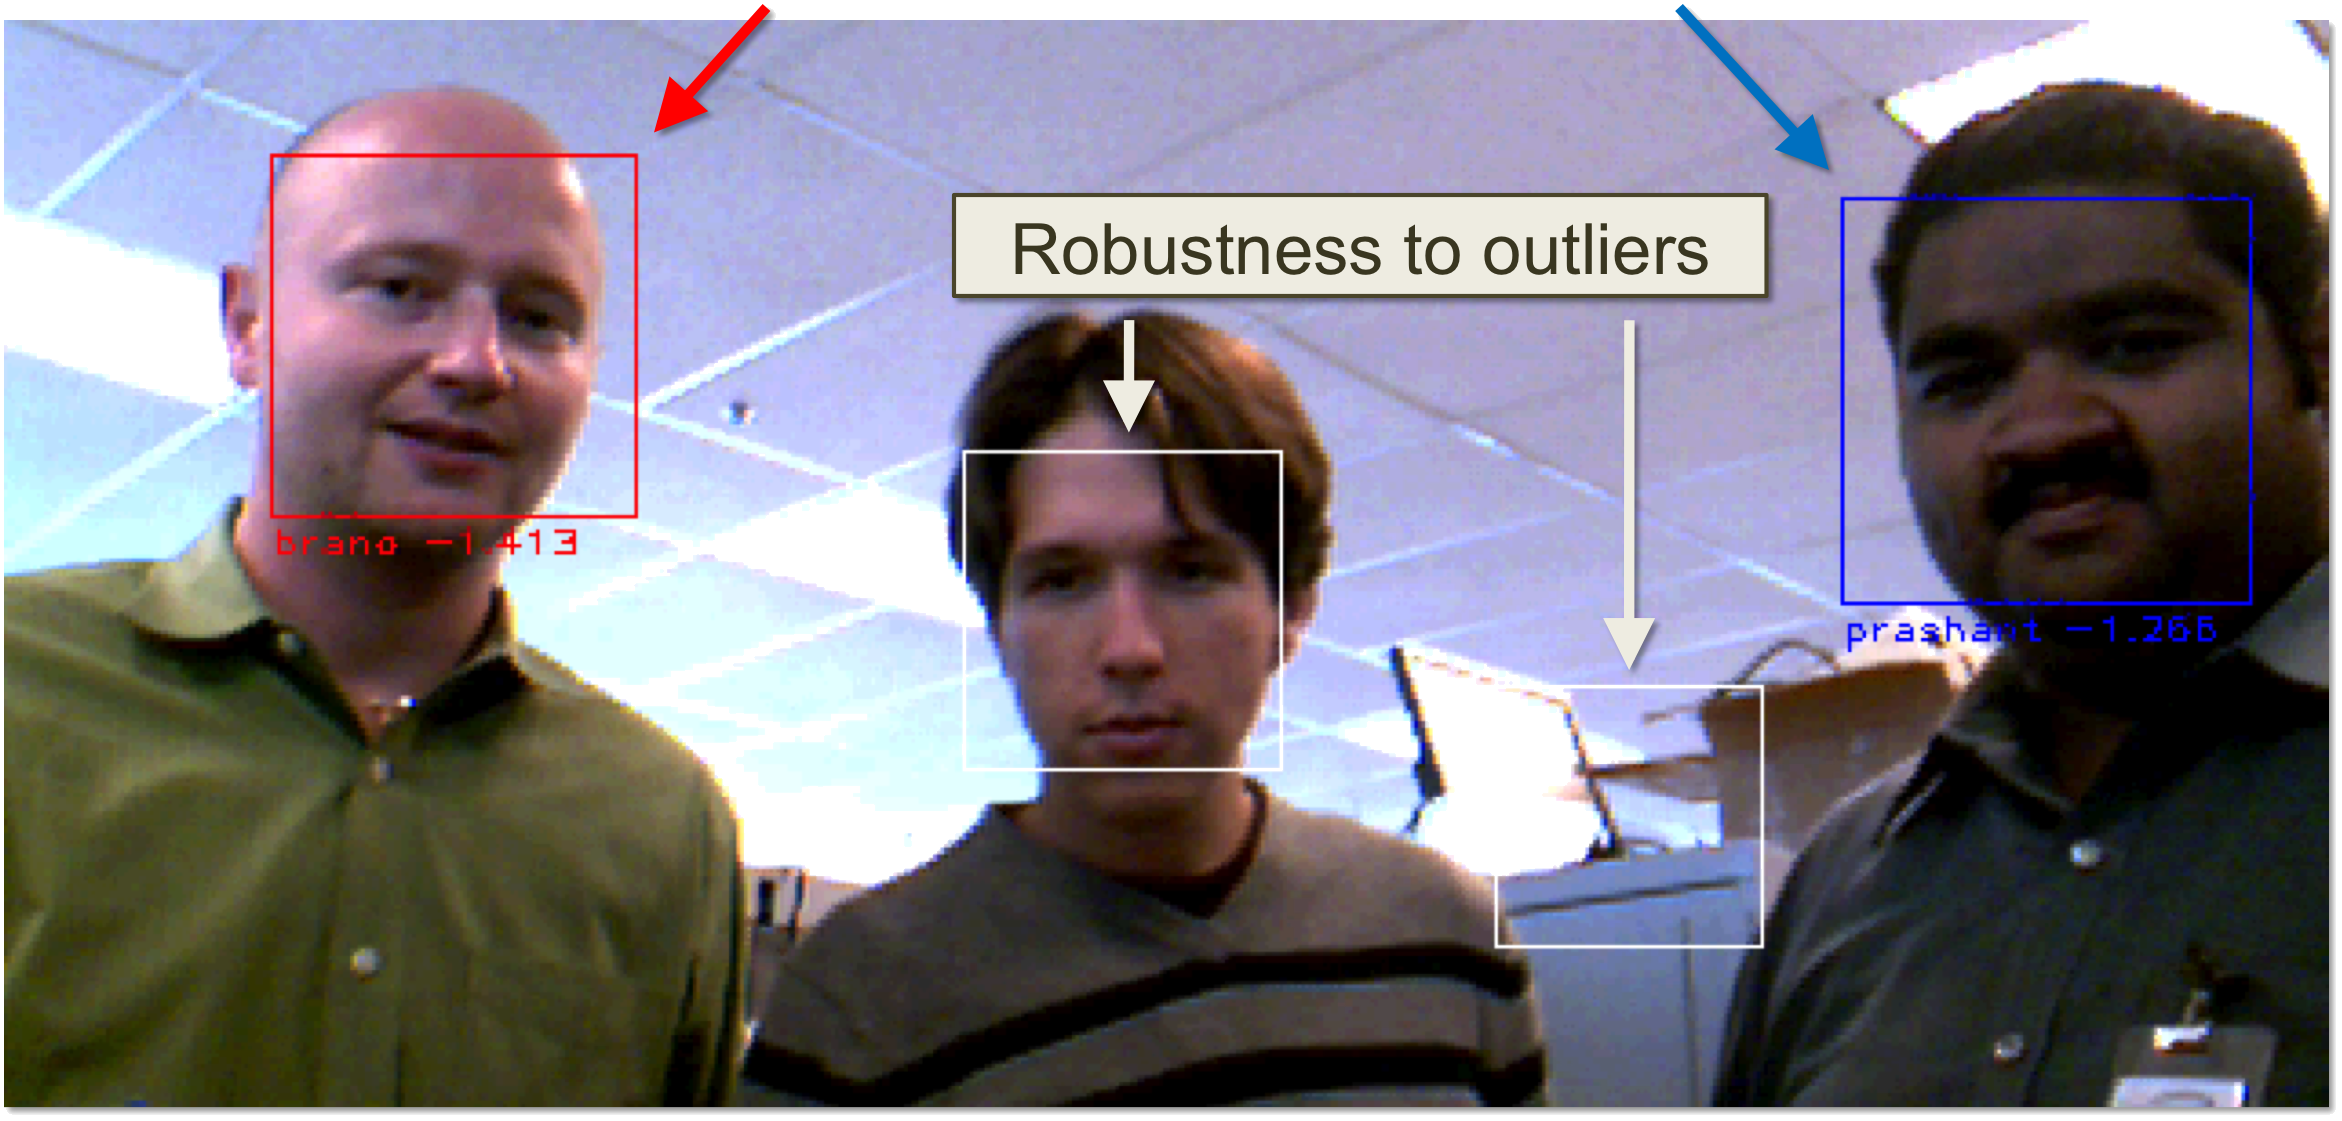
\includegraphics[width=\textwidth]{../img/realfaces}\\ {\tiny Source: Tenenbaum et al. (2000)}}%
\only<4|handout:2>{
\textbf{we will construct it!\\[1em]}%
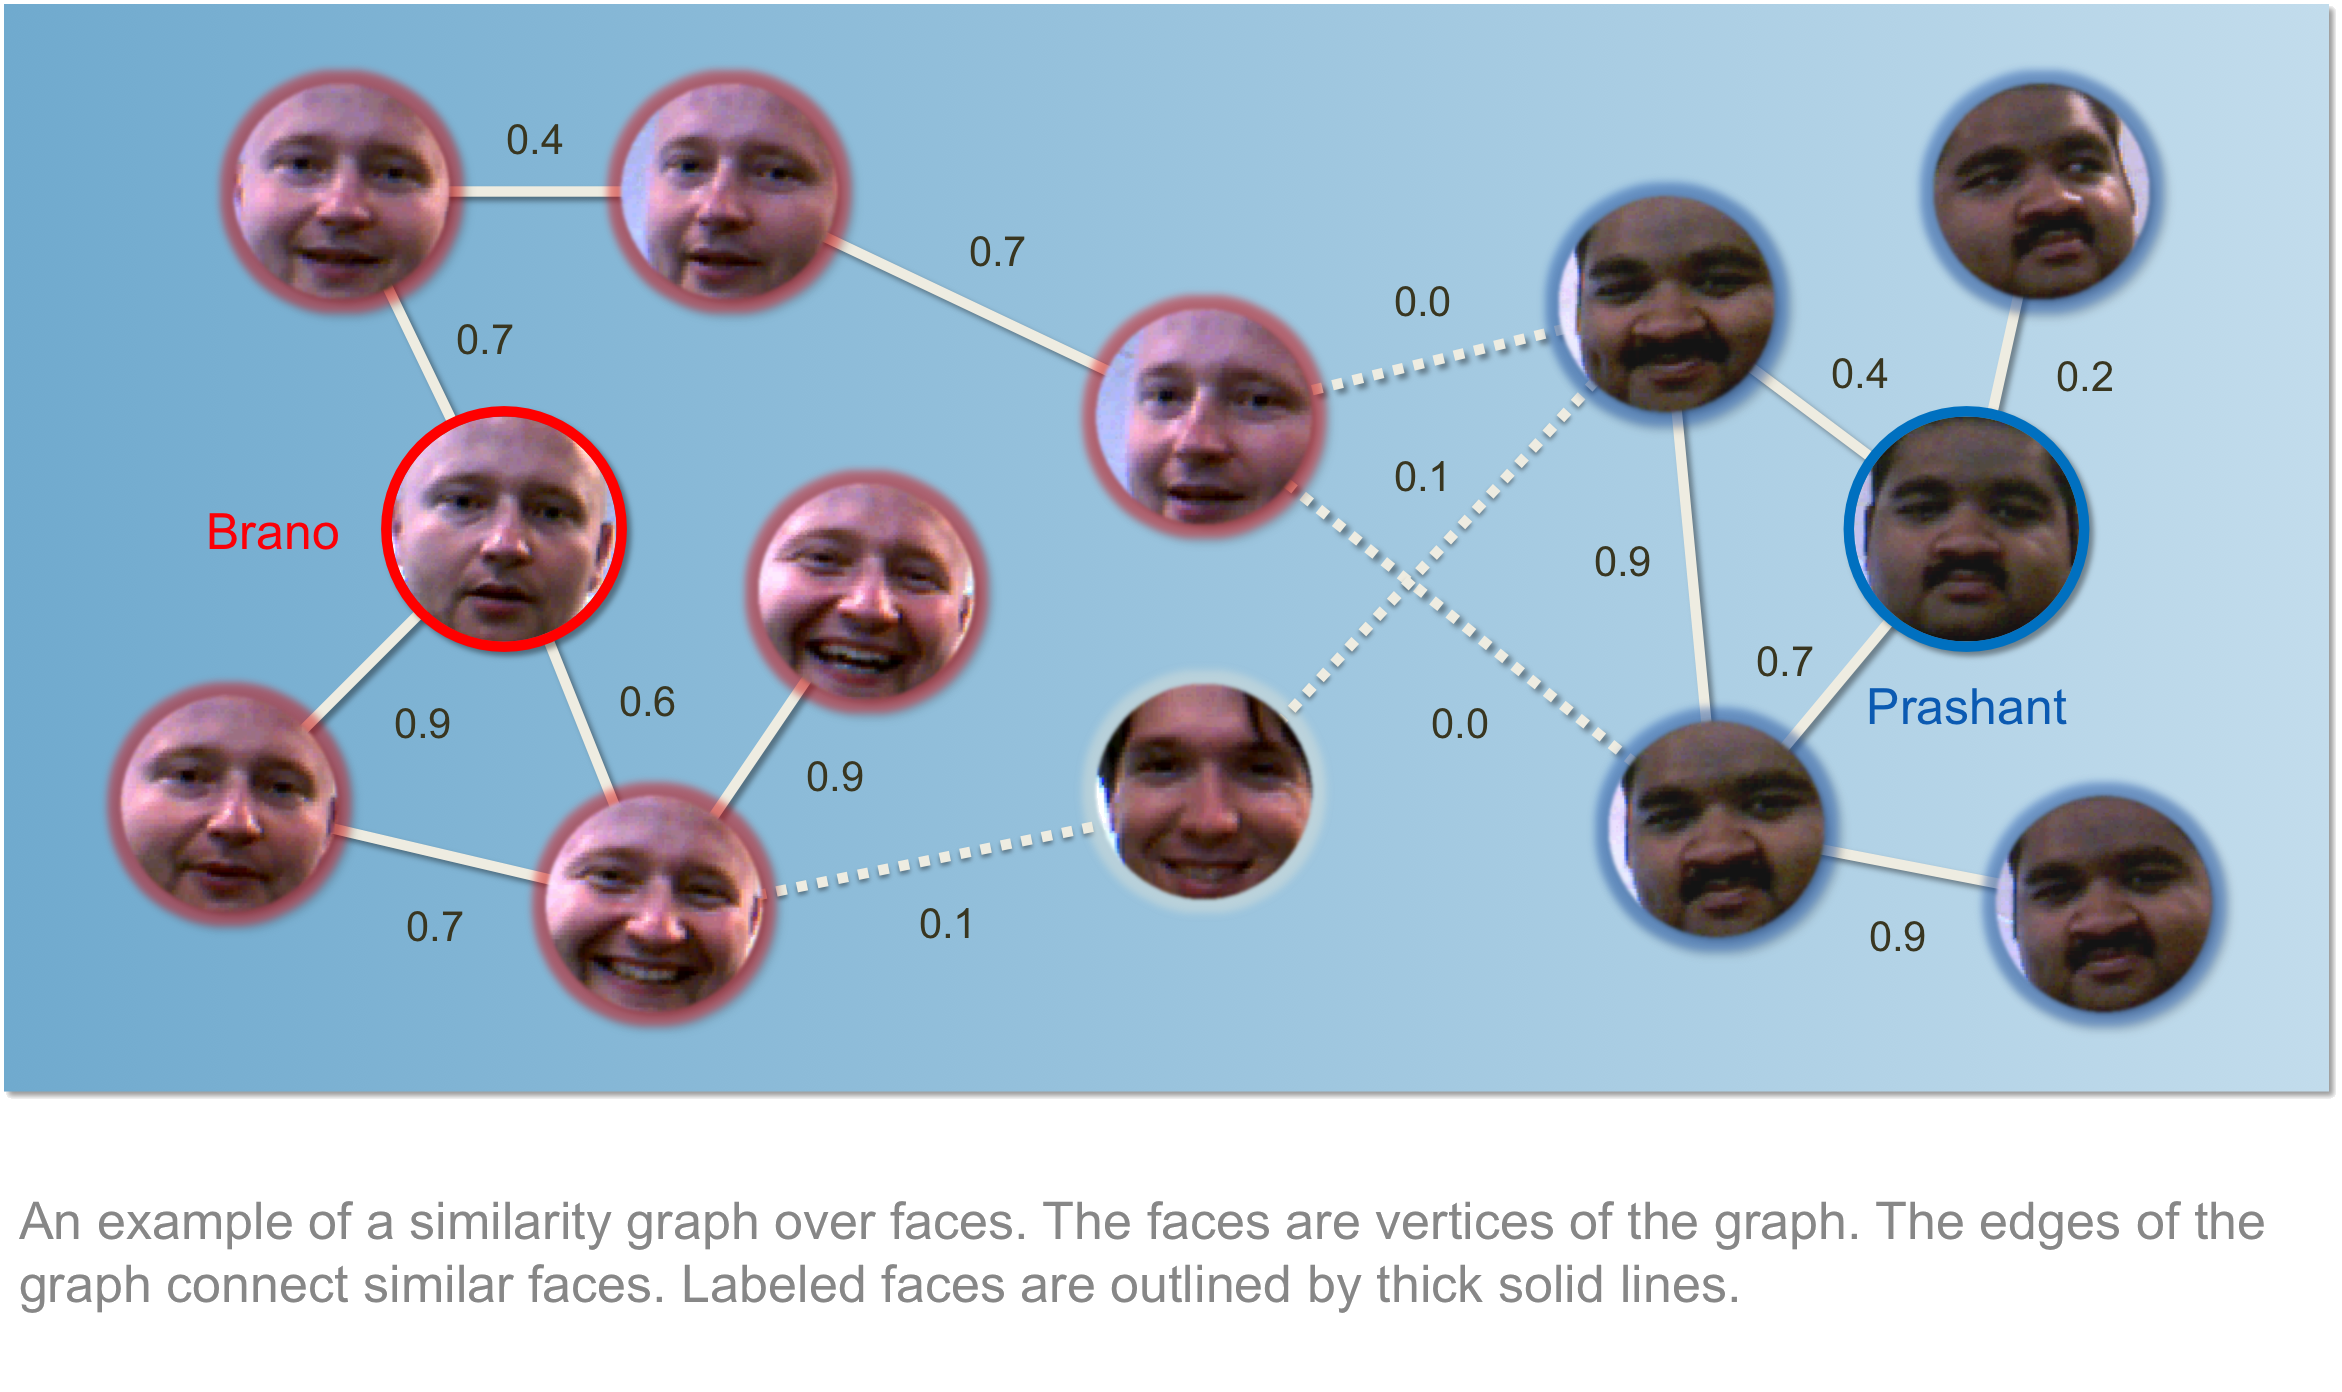
\includegraphics[width=\textwidth]{../img/facegraph}\\ {\tiny Source: Tenenbaum et al. (2000)}}%
\only<2|handout:3>{
\textbf{graph-based semi-supervised learning\\[1em]}%
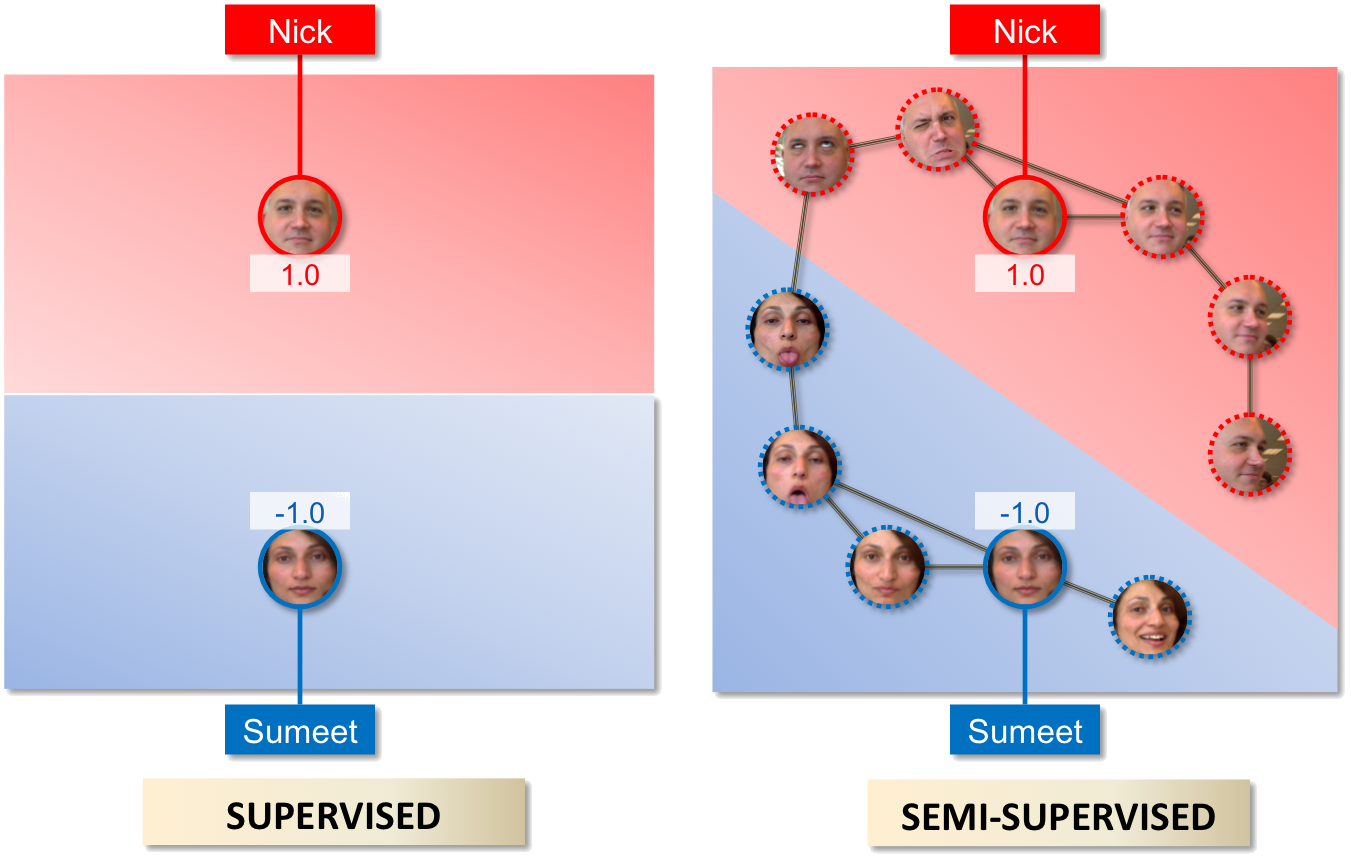
\includegraphics[width=0.8\columnwidth]{../img/ssl}}%
\only<5|handout:4>{
\textbf{online learning - graph sparsification\\[1em]}%
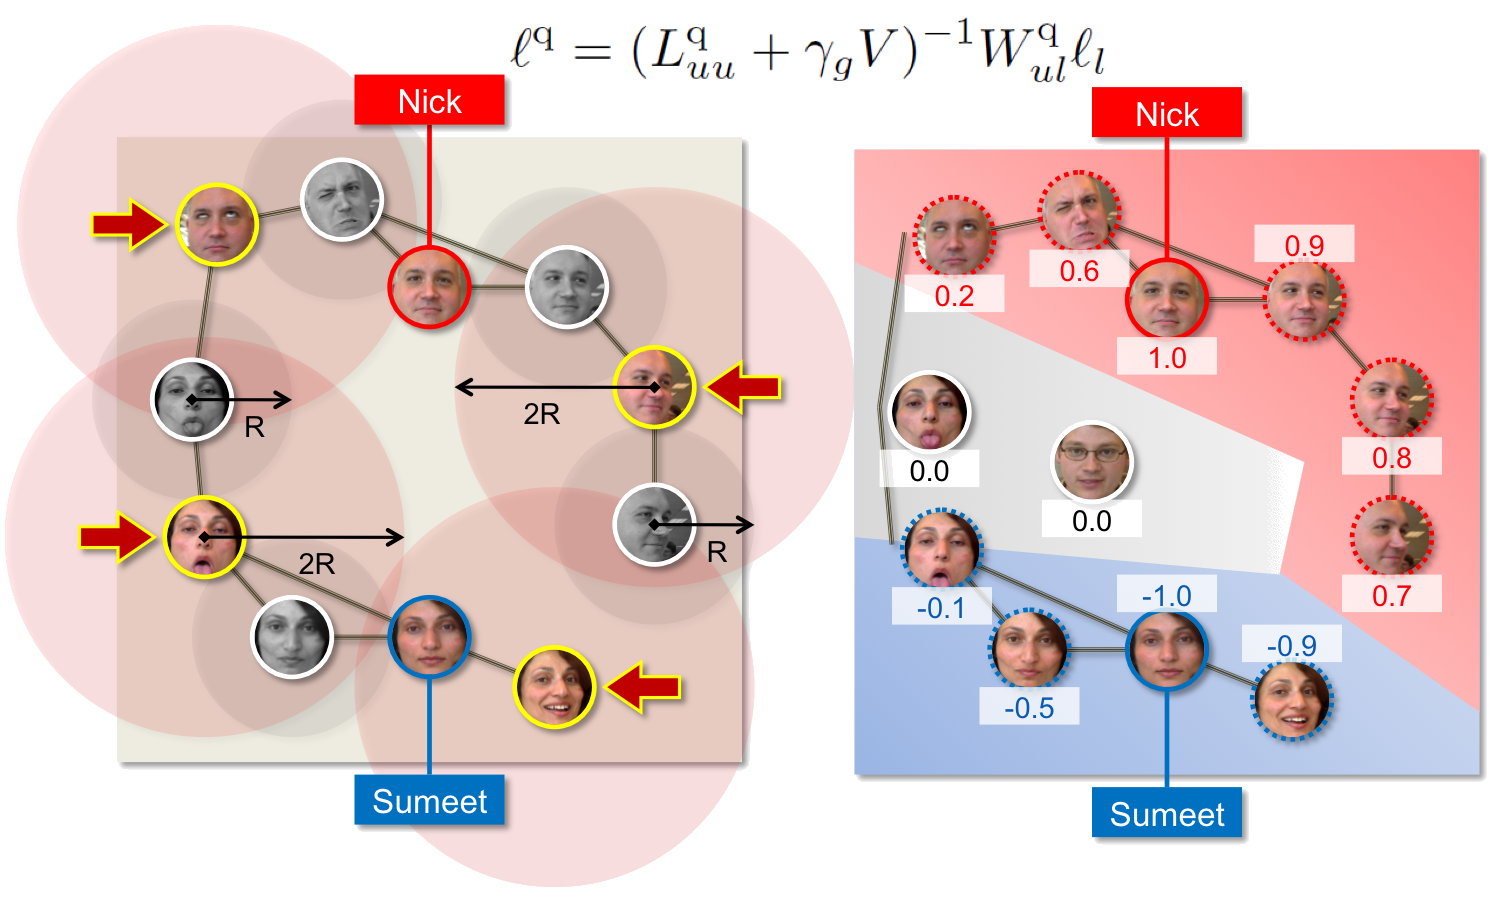
\includegraphics[width=0.8\columnwidth]{../img/charikar}}%
\end{center}
\end{frame}


\begin{frame}
\begin{center}
\textbf{\HUGE DEMO}\\[1em]
%\pause
second TD\\[1em]
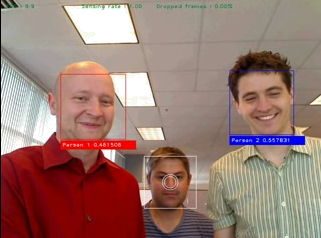
\includegraphics[width=0.3\columnwidth]{../img/demosslface} \hskip 1em
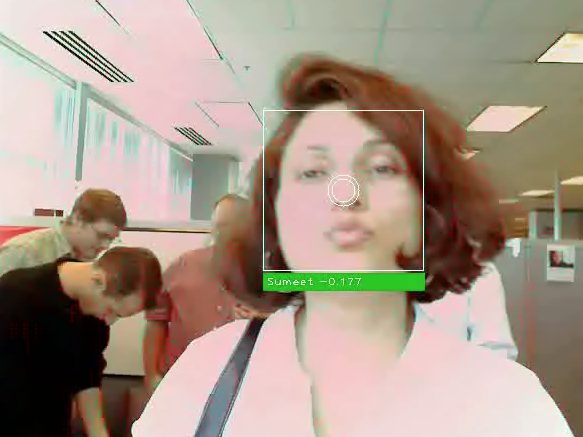
\includegraphics[width=0.3\columnwidth]{../img/demosslface2}\\[1em]%
{\scriptsize \textbf{see the demo:}
\url{https://misovalko.github.io/publications/kveton2009nipsdemo.officespace.mov}\\[1em]
}
\end{center}
\end{frame}

\begin{frame}
\frametitle{OSS FaceReco: Analysis}
\begin{center}
\only<1|handout:1>{
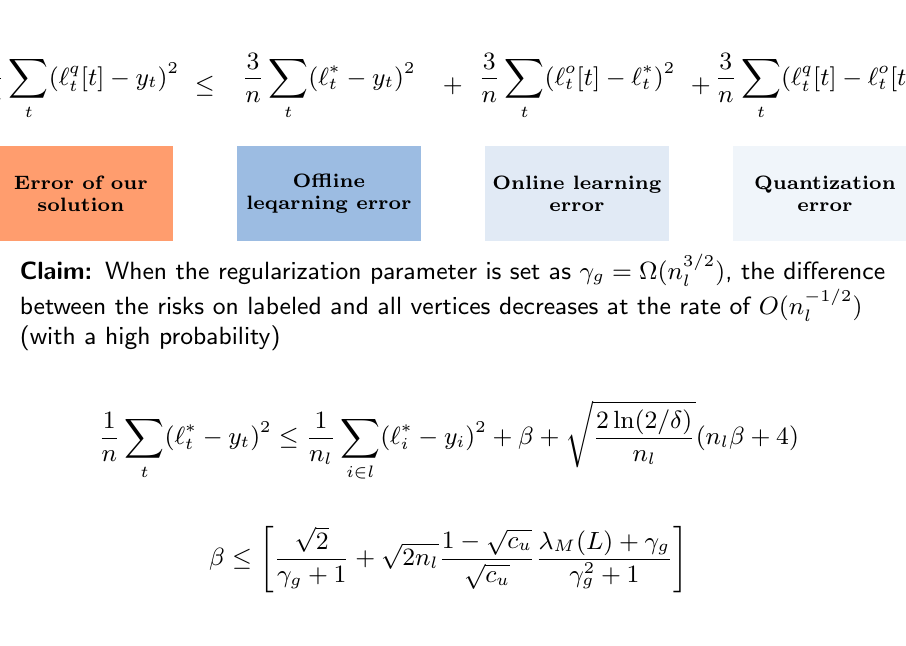
\begin{tikzpicture}[
    x=0.45cm, y=0.5cm,
    font=\sffamily\small,
    eqn/.style={text=black, align=center, anchor=center},
    eqnBottom/.style={text=black, align=center},
    labelbox/.style={
        rectangle, 
        minimum height=1.2cm, 
        text width=2.2cm,
        align=center, 
        font=\scriptsize\bfseries,
        inner sep=2pt,
        anchor=north
    }
]
    % --- BOUNDING BOX ---
    \useasboundingbox (-12, -10) rectangle (12, 5);

    % --- TOP EQUATION (Spaced Out) ---
    \node[eqn] (lhs)   at (-10.5, 3.5) {$\displaystyle \frac{1}{n} \sum_{t} (\ell_t^q[t] - y_t)^2$};
    \node[eqn] (leq)   at (-7.0, 3.5) {$\leq$};
    \node[eqn] (rhs1)  at (-3.5, 3.5) {$\displaystyle \frac{3}{n} \sum_{t} (\ell_t^* - y_t)^2$};
    \node[eqn] (plus1) at (0, 3.5)    {$+$};
    \node[eqn] (rhs2)  at (3.5, 3.5)  {$\displaystyle \frac{3}{n} \sum_{t} (\ell_t^o[t] - \ell_t^*)^2$};
    \node[eqn] (plus2) at (7.0, 3.5)  {$+$};
    \node[eqn] (rhs3)  at (10.5, 3.5) {$\displaystyle \frac{3}{n} \sum_{t} (\ell_t^q[t] - \ell_t^o[t])^2$};

    % --- COLORED BOXES (Aligned to Terms) ---
    \def\boxY{2.0}
    \node[labelbox, fill=boxOrange] at (-10.5, \boxY) {Error of our\\solution};
    \node[labelbox, fill=boxBlue]   at (-3.5, \boxY) {Offline\\leqarning error};
    \node[labelbox, fill=boxLightBlue, text=black] at (3.5, \boxY) {Online learning\\error};
    \node[labelbox, fill=boxWhite, text=black] at (10.5, \boxY) {Quantization error};
    
    % --- BOTTOM PART ---
    \node[text=black, text width=11cm, anchor=north] (claim) at (0, -0.5) {
        \textbf{Claim:} When the regularization parameter is set as $\gamma_g = \Omega(n_l^{3/2})$, the difference between the risks on labeled and all vertices decreases at the rate of $O(n_l^{-1/2})$ (with a high probability)
    };
    \node[eqnBottom] (botEq1) at (0, -5.5) {
        $\displaystyle \frac{1}{n} \sum_{t} (\ell_t^* - y_t)^2 \leq \frac{1}{n_l} \sum_{i \in l} (\ell_i^* - y_i)^2 + \beta + \sqrt{\frac{2 \ln(2/\delta)}{n_l}} (n_l \beta + 4)$
    };
    \node[eqnBottom] (botEq2) at (0, -8.5) {
        $\displaystyle \beta \leq \left[ \frac{\sqrt{2}}{\gamma_g + 1} + \sqrt{2n_l} \frac{1 - \sqrt{c_u}}{\sqrt{c_u}} \frac{\lambda_M(L) + \gamma_g}{\gamma_g^2 + 1} \right]$
    };
\end{tikzpicture}
}%
\only<2|handout:2>{
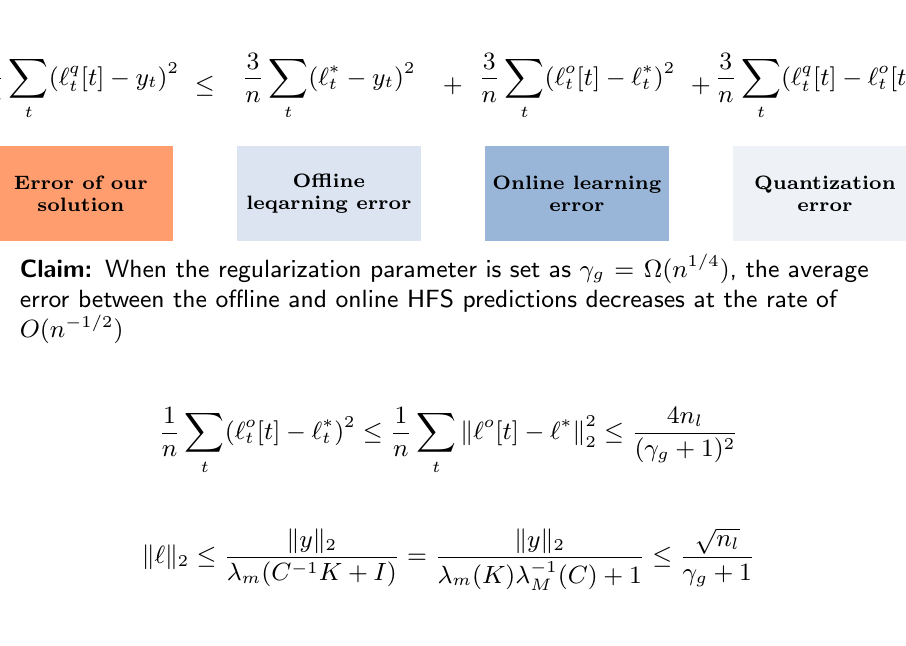
\begin{tikzpicture}[
    x=0.45cm, y=0.5cm,
    font=\sffamily\small,
    eqn/.style={text=black, align=center, anchor=center},
    eqnBottom/.style={text=black, align=center},
    labelbox/.style={
        rectangle, 
        minimum height=1.2cm, 
        text width=2.2cm,
        align=center, 
        font=\scriptsize\bfseries,
        inner sep=2pt,
        anchor=north
    }
]
    % --- BOUNDING BOX ---
    \useasboundingbox (-12, -10) rectangle (12, 5);

    % --- TOP EQUATION ---
    \node[eqn] (lhs)   at (-10.5, 3.5) {$\displaystyle \frac{1}{n} \sum_{t} (\ell_t^q[t] - y_t)^2$};
    \node[eqn] (leq)   at (-7.0, 3.5) {$\leq$};
    \node[eqn] (rhs1)  at (-3.5, 3.5) {$\displaystyle \frac{3}{n} \sum_{t} (\ell_t^* - y_t)^2$};
    \node[eqn] (plus1) at (0, 3.5)    {$+$};
    \node[eqn] (rhs2)  at (3.5, 3.5)  {$\displaystyle \frac{3}{n} \sum_{t} (\ell_t^o[t] - \ell_t^*)^2$};
    \node[eqn] (plus2) at (7.0, 3.5)  {$+$};
    \node[eqn] (rhs3)  at (10.5, 3.5) {$\displaystyle \frac{3}{n} \sum_{t} (\ell_t^q[t] - \ell_t^o[t])^2$};

    % --- COLORED BOXES ---
    \def\boxY{2.0}
    \node[labelbox, fill=boxOrange] at (-10.5, \boxY) {Error of our\\solution};
    \node[labelbox, fill=b2Box2]    at (-3.5, \boxY) {Offline\\leqarning error};
    \node[labelbox, fill=b2Box3]    at (3.5, \boxY)  {Online learning\\error};
    \node[labelbox, fill=b2Box4, text=black] at (10.5, \boxY) {Quantization error};
    
    % --- BOTTOM PART ---
    \node[text=black, text width=11cm, anchor=north] (claim) at (0, -0.5) {
        \textbf{Claim:} When the regularization parameter is set as $\gamma_g = \Omega(n^{1/4})$, the average error between the offline and online HFS predictions decreases at the rate of $O(n^{-1/2})$
    };
    \node[eqnBottom] (botEq1) at (0, -5.5) {
        $\displaystyle \frac{1}{n} \sum_{t} (\ell_t^o[t] - \ell_t^*)^2 \leq \frac{1}{n} \sum_{t} \left\| \ell^o[t] - \ell^* \right\|_2^2 \leq \frac{4n_l}{(\gamma_g + 1)^2}$
    };
    \node[eqnBottom] (botEq2) at (0, -8.5) {
        $\displaystyle \|\ell\|_2 \leq \frac{\|y\|_2}{\lambda_m(C^{-1}K + I)} = \frac{\|y\|_2}{\lambda_m(K)\lambda_M^{-1}(C) + 1} \leq \frac{\sqrt{n_l}}{\gamma_g + 1}$
    };
\end{tikzpicture}
}%
\only<3|handout:3>{
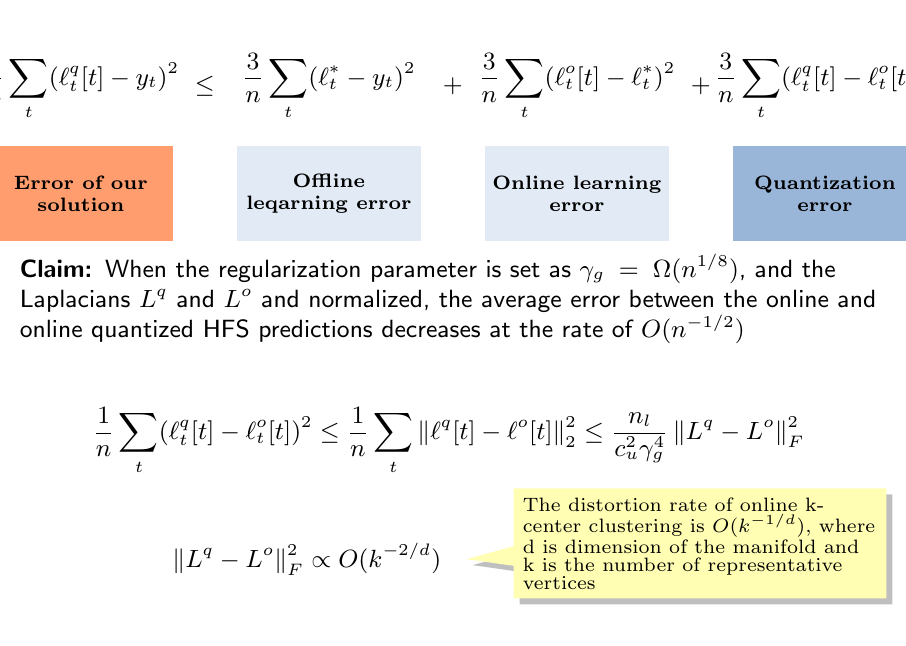
\begin{tikzpicture}[
    x=0.45cm, y=0.5cm,
    font=\sffamily\small,
    eqn/.style={text=black, align=center, anchor=center},
    eqnBottom/.style={text=black, align=center},
    labelbox/.style={
        rectangle, 
        minimum height=1.2cm, 
        text width=2.2cm,
        align=center, 
        font=\scriptsize\bfseries,
        inner sep=2pt,
        anchor=north
    }
]
    % --- BOUNDING BOX ---
    \useasboundingbox (-12, -10) rectangle (12, 5);

    % --- TOP EQUATION ---
    \node[eqn] (lhs)   at (-10.5, 3.5) {$\displaystyle \frac{1}{n} \sum_{t} (\ell_t^q[t] - y_t)^2$};
    \node[eqn] (leq)   at (-7.0, 3.5) {$\leq$};
    \node[eqn] (rhs1)  at (-3.5, 3.5) {$\displaystyle \frac{3}{n} \sum_{t} (\ell_t^* - y_t)^2$};
    \node[eqn] (plus1) at (0, 3.5)    {$+$};
    \node[eqn] (rhs2)  at (3.5, 3.5)  {$\displaystyle \frac{3}{n} \sum_{t} (\ell_t^o[t] - \ell_t^*)^2$};
    \node[eqn] (plus2) at (7.0, 3.5)  {$+$};
    \node[eqn] (rhs3)  at (10.5, 3.5) {$\displaystyle \frac{3}{n} \sum_{t} (\ell_t^q[t] - \ell_t^o[t])^2$};

    % --- COLORED BOXES ---
    \def\boxY{2.0}
    \node[labelbox, fill=boxOrange] at (-10.5, \boxY) {Error of our\\solution};
    \node[labelbox, fill=b3Box2, text=black] at (-3.5, \boxY) {Offline\\leqarning error};
    \node[labelbox, fill=b3Box3, text=black] at (3.5, \boxY)  {Online learning\\error};
    \node[labelbox, fill=b3Box4]    at (10.5, \boxY)  {Quantization error};
    
    % --- BOTTOM PART ---
    \node[text=black, text width=11cm, anchor=north] (claim) at (0, -0.5) {
        \textbf{Claim:} When the regularization parameter is set as $\gamma_g = \Omega(n^{1/8})$, and the Laplacians $L^q$ and $L^o$ and normalized, the average error between the online and online quantized HFS predictions decreases at the rate of $O(n^{-1/2})$
    };
    \node[eqnBottom] (botEq1) at (0, -5.5) {
        $\displaystyle \frac{1}{n} \sum_{t} (\ell_t^q[t] - \ell_t^o[t])^2 \leq \frac{1}{n} \sum_{t} \left\| \ell^q[t] - \ell^o[t] \right\|_2^2 \leq \frac{n_l}{c_u^2 \gamma_g^4} \left\| L^q - L^o \right\|_F^2$
    };
    \node[eqnBottom] (botEq2) at (-4, -8.5) {
        $\displaystyle \left\| L^q - L^o \right\|_F^2 \propto O(k^{-2/d})$
    };

    % Callout
    \node[rectangle callout, 
          callout absolute pointer={($(botEq2.east)+(0.2,0)$)},
          fill=calloutYellow, 
          draw=none,
          drop shadow,
          align=left, 
          text width=4.5cm, 
          font=\scriptsize\linespread{0.8}\selectfont,
          anchor=west] at (1.7, -8.1) {
        The distortion rate of online k-center clustering is $O(k^{-1/d})$, where d is dimension of the manifold and k is the number of representative vertices
    };
\end{tikzpicture}
}%
\end{center}
\end{frame}

\usebackgroundtemplate{%
\tikz\node[opacity=0.05] {%
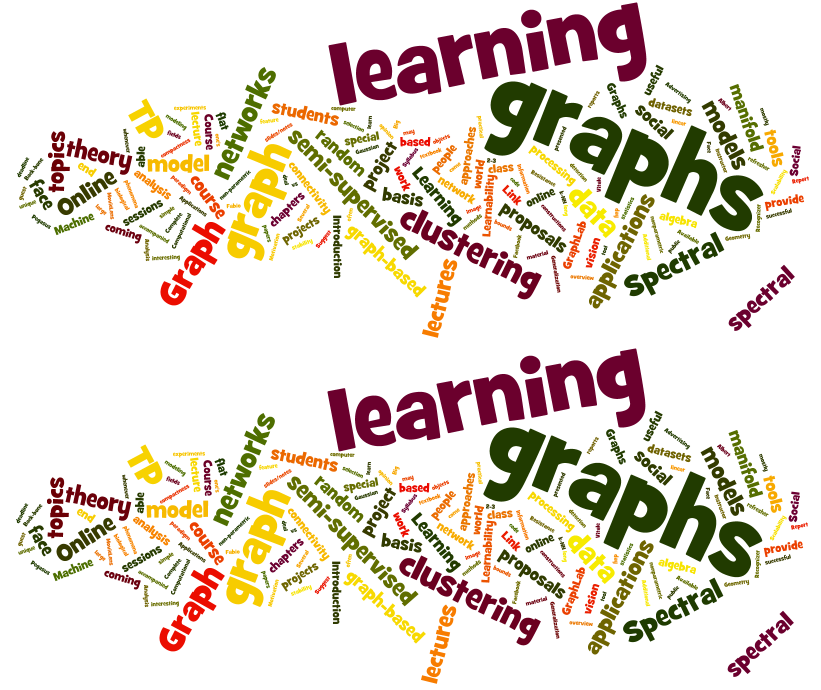
\includegraphics[width=\paperwidth]{../img/wordle2}
};}

%\section{Other topics}
%\begin{frame}
%\frametitle{\textbf{Some of the other topics}}
%\begin{center}
%\begin{itemize}[<+-| alert@+>]\addtolength{\itemsep}{0.3\baselineskip}
%\item spectral graph theory,  graph Laplacians, spectral clustering
%\item semi-supervised learning and manifold learning
%\item learnability on graphs - transductive learning
%\item online decision-making on graphs, graph bandits
%\item submodularity on graphs
%\item real-world graphs scalability and approximations
%\item spectral sparsification
%\item social network and recommender systems applications
%\item link prediction/link clasification 
%\item signed networks (eOpinions)
%\item generalization bounds by perturbation analysis
%\end{itemize}
%%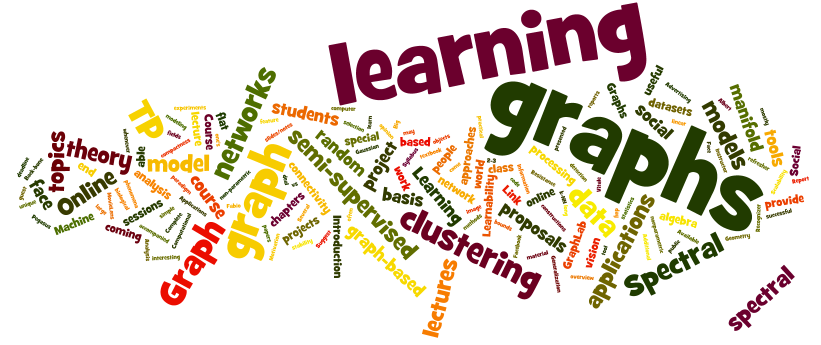
\includegraphics[width=1.08\columnwidth]{../img/wordle}
%\end{center}
%\end{frame}

\usebackgroundtemplate{}



%\section{Administrivia}

\begin{frame}
\frametitle{MVA and Graphs: 2 courses}
\onslide<1,2|handout:1>{
\vskip -0.5cm
{\small The two MVA graph courses offer complementary material.} \\
\vskip 0.5cm
}
\onslide<1,2|handout:1>{
\begin{columns}
\begin{column}{.5\textwidth}
Fall: \yellcol{\textbf{Graphs in ML}} 
\begin{itemize}
\item[] \emph{this class}
\item focus on learning
\item spectral clustering 
\item random walks
\item graph Laplacian
\item semi-supervised learning
\item theoretical analyses
\item online learning
\item recommender systems
\item \textbf{graph neural networks}
\end{itemize}
\end{column}
}
\onslide<2|handout:1>{
\begin{column}{.5\textwidth}
Late Fall: \yellcol{\textbf{ALTeGraD}}
\begin{itemize}
\item[] \emph{by Michalis Vazirgiannis}
\item dimensionality reduction
\item feature selection
\item text mining
\item graph mining
\item community mining 
\item graph generators
\item graph-evaluation measures 
\item privacy in graph mining
\item big data
\end{itemize}
\end{column}
}
\end{columns}
\end{frame}

\begin{frame}

\frametitle{Administrivia}

\textbf{8 lectures + 3 recitations (TDs)}\\[0.5em]

\textbf{Validation:} grades from TDs (40\%) + class project (60\%) \\[0.7em]

\textbf{Prerequisites:} linear algebra, basic statistics \\[0.7em]

\textbf{Language:} English \\[0.7em]

\textbf{Course website:}\\[-0.5em]
{\scriptsize\url{https://misovalko.github.io/mva-ml-graphs.html}} \\[0.5em]


%\textbf{Contact:}\\
%{\scriptsize
%Lecturer: Michal.Valko @ inria.fr\\[-0.5em]
%TA: Daniele.Calandriello @ inria.fr 
%}
\end{frame}


%\begin{frame}
%\frametitle{First class on  Wednesday, October 3th at \alert{14:00}!}
%%\vspace{0.2in}
%\begin{center}
%%\vspace{0.1in}
%%{\LARGE Course starts Monday, September 28th at 11 am!}
%\tikz{
    %\node[anchor=south west, inner sep=0] (image) at (0,0) {
    %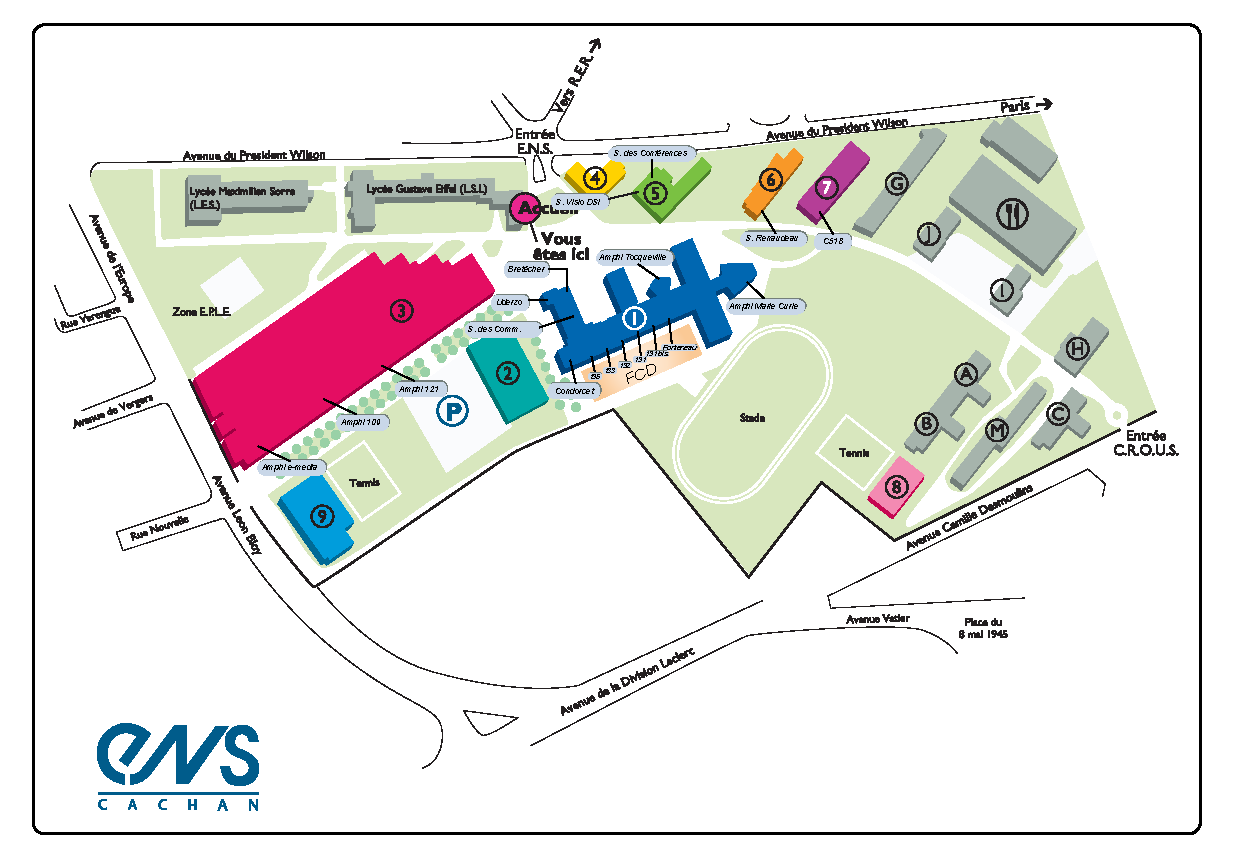
\includegraphics[width=9cm]{../img/salles-campus.pdf}
    %};
    %\begin{scope}[x={(image.south east)},y={(image.north west)}]
        %\draw [-stealth, line width=5pt, mvaHighlight] (0.5,0.3) -- (0.47,0.54);
        %%\draw [-stealth, line width=5pt, mvaHighlight] (0.5,0.3) -- (0.60,0.64);
    %\end{scope}
%}
%\end{center}
%\end{frame}

\MakeLastSlide


\end{document}


